\documentclass[11pt,a4paper]{article}


% font
%\usepackage{fontspec}
%\setmainfont{Times New Roman}
%\usepackage{tgschola}

\usepackage{helvet}
\renewcommand{\familydefault}{\sfdefault}

\usepackage[margin=0.8in]{geometry}
\usepackage[utf8]{inputenc}
\usepackage{amsmath}
\usepackage{amsfonts}
\usepackage{amssymb}

% https://www.sharelatex.com/learn/Hyperlinks
\usepackage{hyperref}
\hypersetup{
    colorlinks=true,
    linkcolor=blue9,
    filecolor=magenta,      
    urlcolor=red,
}
 
\usepackage{float}

\usepackage{lipsum}% http://ctan.org/pkg/lipsum

%% Bibliography/references packages
\usepackage[comma]{natbib}
%%\bibliographystyle{agsm}
\bibliographystyle{dcu}

%% https://en.wikibooks.org/wiki/LaTeX/List_Structures
\usepackage{scrextend}

% tables, row colour
\usepackage{tabularx,colortbl}
% For vertical centering text in X column
\renewcommand\tabularxcolumn[1]{m{#1}}

% https://tex.stackexchange.com/questions/22751/how-to-force-table-caption-on-top
%\usepackage[tableposition=top]{caption}
\usepackage{float}
\floatstyle{plaintop}
\restylefloat{table}

% https://en.wikibooks.org/wiki/LaTeX/List_Structures
\usepackage{enumitem}

% https://jansoehlke.com/2010/06/strikethrough-in-latex/
\usepackage{ulem}

% Code highlighting
\usepackage[outputdir=build]{minted}

%% Report variables
\newcommand{\scname}{PRCO304}
\newcommand{\dlatestv}{1.00}


\definecolor{babyblueeyes}{rgb}{0.63, 0.79, 0.95}
\definecolor{ballblue}{rgb}{0.13, 0.67, 0.8}
\definecolor{beaublue}{rgb}{0.74, 0.83, 0.9}
\definecolor{blue8}{rgb}{0.09, 0.39, 0.67}
\definecolor{blue9}{rgb}{0.00, 0.30, 0.51}
\definecolor{blue9d}{rgb}{0.00, 0.21, 0.36}


%\usepackage{etoolbox}
%\patchcmd{\chapter}{\thispagestyle{plain}}{\thispagestyle{fancy}}{}{}

%https://tex.stackexchange.com/questions/75667/change-colour-on-chapter-section-headings-lyx
\usepackage{sectsty}
\chapterfont{\color{blue9d}}
\sectionfont{\color{blue9d}}
\subsectionfont{\color{blue9d}}
%\allchapterfont{\itshape}

\usepackage{titlesec}

\usepackage{array,booktabs,arydshln,xcolor}
\usepackage{xcolor}% http://ctan.org/pkg/xcolor
\usepackage{fancyhdr}% http://ctan.org/pkg/fancyhdr
\fancypagestyle{plain}{%
	\renewcommand{\headrulewidth}{3pt}
	\renewcommand{\headrule}{\hbox to\headwidth{%
		\color{blue9}\leaders\hrule height \headrulewidth\hfill}}
	\renewcommand{\footrulewidth}{3pt}
	\renewcommand{\footrule}{\hbox to\headwidth{%
		\color{blue9}\leaders\hrule height \headrulewidth\hfill}}
	
	%\fancyhf{}
	%\fancyhead[LE]{\textbf{\leftmark}}
	%\fancyhead[RE]{\textbf{\scname{}}}
	%\fancyhead[LO]{\textbf{\scname{}}}
	%\fancyhead[RO]{\textbf{\rightmark}}

	%\fancyfoot[LE]{\textbf{\thepage}}
	%\fancyfoot[RE]{\textbf{\scname{} Configuration Guide}}
	%\fancyfoot[LO]{\textbf{\scname{} Configuration Guide}}
	%\fancyfoot[RO]{\textbf{\thepage}}
}


%% Make bibliography show in table of contents
%% https://tex.stackexchange.com/questions/8458/making-the-bibliography-appear-in-the-table-of-contents
\usepackage[nottoc,numbib]{tocbibind}
%% ^^^ overwrites \bibname, so set it back
\renewcommand{\bibname}{References}

\RequirePackage{filecontents}
\begin{filecontents}{vmicro16.bib}

\end{filecontents}

%s comments
\usepackage{verbatim}

%inline graphs
\usepackage{wrapfig}
% multiple figures on line
\usepackage{subfig}

\usepackage{graphicx}
\graphicspath{ {img/} }

% Caption font size
% https://tex.stackexchange.com/questions/86120/font-size-of-figure-caption-header
\usepackage[font=scriptsize,labelfont=bf]{caption}

%\setlength{\belowcaptionskip}{-10pt}
%\setlength{\abovecaptionskip}{-5pt} % Chosen fairly arbitrarily


\usepackage{fancyhdr}
\pagestyle{fancy}
\lhead{\rightmark}
\chead{}
\rhead{Highlight Report Document (Rev. \dlatestv{})}
\lfoot{Page \thepage}
\cfoot{}
\rfoot{Ben Lancaster 201280376}

\renewcommand{\subsectionmark}[1]{\markright{\thesubsection\ #1}}


\begin{document}

\begin{titlepage}
\begin{center}

\vspace*{5cm}
\Large
\textbf{
%%PRCO304 - Project Initiation Document
%Highlight Reports
{\color{blue9d}Weekly Highlight Report Document (Rev. \dlatestv{})}
}

\vspace{0.4cm}
\large
ELEC5881M -- Multi-core RISC Processor Design

\vspace{4cm}
\textbf{Ben Lancaster 201280376}\\
MSc (Eng) Embedded Systems Engineering

\vspace{4cm}
\today 


\end{center}

\end{titlepage}

\pagestyle{plain}

\section*{Revision History}
\begin{table}[h]
\def\arraystretch{1.5}%  1 is the default, change whatever you need
    \begin{tabularx}{\textwidth}{|l|l|X|}
    \hline
    Date & Week & Changes \\
	\specialrule{2pt}{-2pt}{0pt}
	03/03/2019 & 1 & Week 2 report. \\ \hline
	25/02/2019 & 1 & Initial week 1 report. \\ \hline
    \end{tabularx}
    \caption{Document revisions.}
\end{table}
\newpage

\renewcommand*\contentsname{Table of Contents}

{\hypersetup{linkcolor=black}
\tableofcontents
}

\newpage
\section{Weekly Reports}
\subsection{Weekly Report 5}
\begin{table}[H]
\def\arraystretch{1.5}%  1 is the default, change whatever you need
    \begin{tabularx}{\textwidth}{|X|p|}
    \hline 
	\multicolumn{1}{|c|}{\textbf{Weekly Report 5 -- 25/03/19}}
    \\ \specialrule{2pt}{-2pt}{0pt}	
	\textbf{Active project stage:}\\
	(ON-TIME) Stage 2.3 -- (CORE) Local memory impl \& integration \\
	(ON-TIME) Stage 3.1 -- (CORE) Memory mapped register layout \\
	(ON-TIME) Stage 8.0 -- (CORE) Final Report \\
	
	\\ \hline
	\textbf{Review of work undertaken:}\newline
	Minimal contributions to the project have been made due to high workload and demand from other modules.
	\\	
	\textbf{(EARLY) Stage 8.0 -- (CORE) Final Report}\newline
	Some work has been started on the interim report. 
	
	\\ \hline
	\textbf{Risks and Challenges:}\\
	{\color{red} RC2: Multiple tests and deadlines for other modules.}
	\\ \hline
	
	\textbf{Plan of work for the next week:}\newline
	Next weeks goals are the same as this weeks due to RC2.
	\\
    Stage 2.3 -- (CORE) Local memory impl \& integration\newline
    Stage 3.1 -- (CORE) Memory mapped register layout
	\\ \hline
	
	
	\textbf{Date(s) of supervisory meeting(s) since last Highlight:}\newline
	19/03/19 -- Weekly highlight meeting (skipped due to other commitments).
	\\ \hline
	
	
	\textbf{Notes from supervisory meeting(s) held since last Highlight:}\newline
	/
	\\ \hline
    \end{tabularx}
    %\caption{Document revisions.}
\end{table}
\newpage

\subsection{Weekly Report 4}
\begin{table}[H]
\def\arraystretch{1.5}%  1 is the default, change whatever you need
    \begin{tabularx}{\textwidth}{|X|p|}
    \hline 
	\multicolumn{1}{|c|}{\textbf{Weekly Report 4 -- 18/03/19}}
    \\ \specialrule{2pt}{-2pt}{0pt}	
	\textbf{Active project stage:}\\
	(ON-TIME) Stage 2.3 -- (CORE) Local memory impl \& integration \\
	(ON-TIME) Stage 3.1 -- (CORE) Memory mapped register layout \& impl \\
	
	\\ \hline
	\textbf{Review of work undertaken:}\newline
	Minimal contributions to the project have been made due to high workload and demand from other modules.
	
	\\ \hline
	\textbf{Risks and Challenges:}\\
	{\color{red} RC2: Multiple tests and deadlines for other modules.}
	\\ \hline
	
	\textbf{Plan of work for the next week:}\newline
	Next weeks goals are the same as this weeks due to RC2.
	\\
    Stage 2.3 -- (CORE) Local memory impl \& integration\newline
    Stage 3.1 -- (CORE) Memory mapped register layout
	\\ \hline
	
	
	\textbf{Date(s) of supervisory meeting(s) since last Highlight:}\newline
	12/03/19 -- Weekly highlight meeting (skipped due to other commitments).
	\\ \hline
	
	
	\textbf{Notes from supervisory meeting(s) held since last Highlight:}\newline
	/
	\\ \hline
    \end{tabularx}
    %\caption{Document revisions.}
\end{table}
\newpage

\subsection{Weekly Report 3}
\begin{table}[H]
\def\arraystretch{1.5}%  1 is the default, change whatever you need
    \begin{tabularx}{\textwidth}{|X|p|}
    \hline 
	\multicolumn{1}{|c|}{\textbf{Weekly Report 3 -- 11/03/19}}
    \\ \specialrule{2pt}{-2pt}{0pt}	
	\textbf{Active project stage:}\\
	(ON-TIME) Stage 2.3 -- (CORE) Local memory impl \& integration \\
	(ON-TIME) Stage 3.1 -- (CORE) Memory mapped register layout \& impl \\
	
	\\ \hline
	\textbf{Review of work undertaken:}\newline
	Minimal contributions to the project have been made due to high workload and demand from other modules.
	
	\\ \hline
	\textbf{Risks and Challenges:}\\
	{\color{red} RC2: Multiple tests and deadlines for other modules.}
	\\ \hline
	
	\textbf{Plan of work for the next week:}\newline
	Next weeks goals are the same as this weeks due to RC2.
	\\
    Stage 2.3 -- (CORE) Local memory impl \& integration.\newline
    Stage 3.1 -- (CORE) Memory mapped register layout.
	\\ \hline
	
	
	\textbf{Date(s) of supervisory meeting(s) since last Highlight:}\newline
	05/03/19 -- Weekly highlight meeting.
	\\ \hline
	
	
	\textbf{Notes from supervisory meeting(s) held since last Highlight:}\newline
	Discussion about time management to allow for time to be spent on other modules.
	\\ \hline
    \end{tabularx}
    %\caption{Document revisions.}
\end{table}
\newpage

\subsection{Weekly Report 2}
\begin{table}[H]
\def\arraystretch{1.5}%  1 is the default, change whatever you need
    \begin{tabularx}{\textwidth}{|X|p|}
    \hline 
	\multicolumn{1}{|c|}{\textbf{Weekly Report 2 -- 03/03/19}}
    \\ \specialrule{2pt}{-2pt}{0pt}	
	\textbf{Active project stage:}\\
	(ON-TIME) Stage 2.3 -- (CORE) Local memory impl \& integration \\
	(ON-TIME) Stage 3.1 -- (CORE) Memory mapped register layout \& impl \\
	
	\\ \hline
	\textbf{Review of work undertaken:}\newline
	\textbf{(ON-TIME) Stage 2.3 -- (CORE) Local memory impl \& integration}\newline
	The new decoder has been integrated into the pipeline and basic instruction sequences have been verified.\\
	
	\textbf{(ON-TIME) Stage 3.1 -- (CORE) Memory mapped register layout}\newline
	An internal wishbone master interface has been implemented and is controlled by the MMU.\newline
	A wishbone slave interface has been added to the inputs/outputs of the SoC module. Interaction between cores is still under design, although it will not use Wishbone.
	
	\\ \hline
	\textbf{Risks and Challenges:}\\
	{\color{red} RC2: Multiple tests and deadlines for other modules.}
	\\ \hline
	
	\textbf{Plan of work for the next week:}\newline
    Stage 2.3 -- (CORE) Local memory impl \& integration\newline
    Stage 3.1 -- (CORE) Memory mapped register layout
	\\ \hline
	
	
	\textbf{Date(s) of supervisory meeting(s) since last Highlight:}\newline
	26/02/19 -- Weekly highlight meeting
	\\ \hline
	
	
	\textbf{Notes from supervisory meeting(s) held since last Highlight:}\newline
	Discussion about target FPGAs: It was decided to target Xilinx Spartan 6 with ISE and Altera Cyclone V with Quartus.
	\\ \hline
    \end{tabularx}
    %\caption{Document revisions.}
\end{table}
\newpage

\subsection{Weekly Report 1}
\begin{table}[H]
\def\arraystretch{1.5}%  1 is the default, change whatever you need
    \begin{tabularx}{\textwidth}{|X|p|}
    \hline 
	\multicolumn{1}{|c|}{\textbf{Weekly Report 1 -- 25/02/19}}
    \\ \specialrule{2pt}{-2pt}{0pt}	
	\textbf{Active project stage:}\\
	(ON-TIME) Stage 1.2 -- (CORE) Stage/Time Allocation Planning \\
	(ON-TIME) Stage 2.1 -- (CORE) Decoder, Register set, impl \& integration \\
	
	\\ \hline
	\textbf{Review of work undertaken:}\newline	
	Project tasks and deliverables have been formalised and broken up into smaller tasks.
	\newline\newline
	\textbf{(ON-TIME) Stage 1.2 -- (CORE) Stage/Time Allocation Planning }\newline
	The project has been broken up into smaller tasks. Each task has been assigned a start date and expected duration. A gantt chart has also been produced. Images of the gantt chart and task list are included in section \ref{sect:week1}.\\
	
	\textbf{(ON-TIME) Stage 2.1 -- (CORE) Decoder, Register set, impl \& integration}\newline
	The new decoder for the new ISA has been built and has been somewhat integrated into the pipeline through the \verb|vmicro16_idex| module.
	
	\\ \hline
	\textbf{Risks and Challenges:}\\
	{\color{gray} Resolved risks:\newline
	RC1 -- Project planning not adequately performed. The project should be broken down into smaller tasks and each task should be assigned a priority and timeslot.}
	\\ \hline
	
	
	\textbf{Plan of work for the next week:}\newline
    Stage 2.1 -- Continue integrating the new decoder into the CPU module.
	\\ \hline
	
	
	\textbf{Date(s) of supervisory meeting(s) since last Highlight:}\newline
	19/02/19 -- Weekly highlight meeting
	\\ \hline
	
	
	\textbf{Notes from supervisory meeting(s) held since last Highlight:}\newline
	RC1 -- It was decided to perform a weekly highlight report, which details progress, challenges, and obstacles.
	\\ \hline
    \end{tabularx}
    %\caption{Document revisions.}
\end{table}

\newpage
\section{Weekly Report Attachments}
\subsection{Week 1}
\label{sect:week1}
\begin{figure}[H]
    \centering
    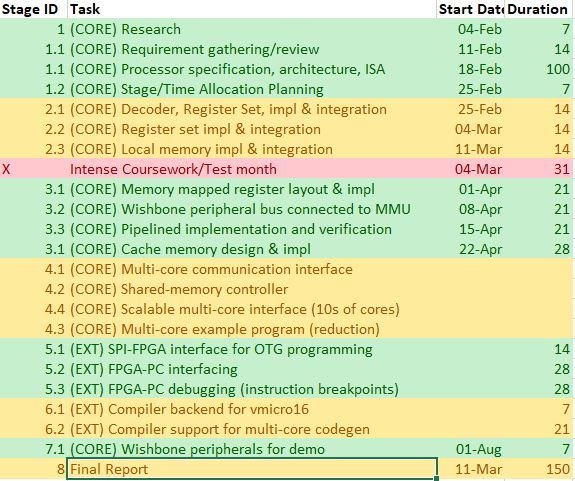
\includegraphics[scale=0.8]{week1_tasks}
    \caption{Deliverables have been formalised and their development has been broken up into stages. Green/yellow colour simply identifies tasks in a new stage.}
    \label{fig:h5_impl}
\end{figure}

\begin{figure}[H]
    \centering
    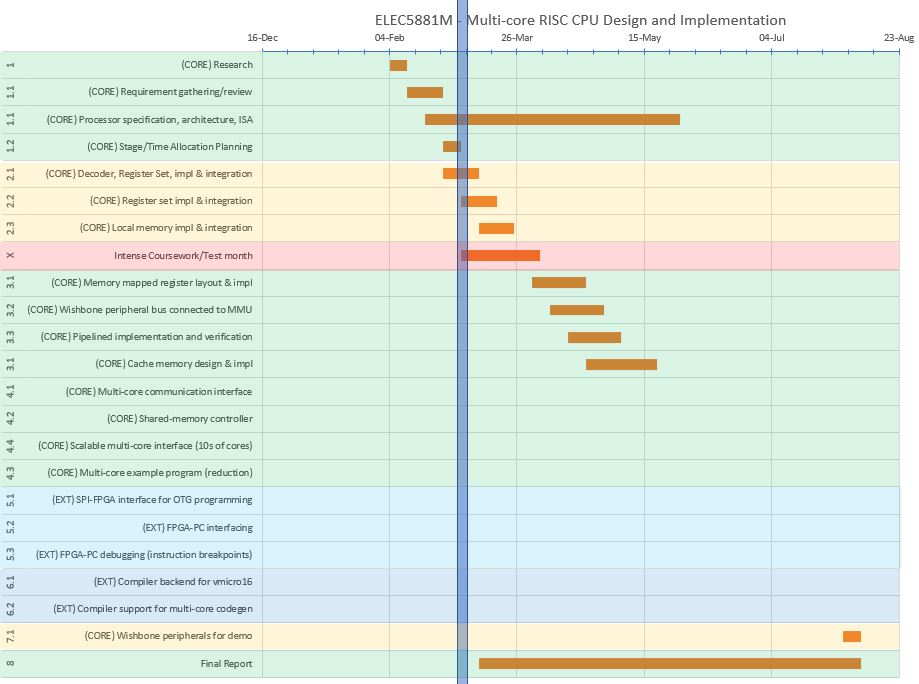
\includegraphics[scale=0.8]{week1_gantt}
    \caption{Visualisation of the stages in a Gantt chart.}
    \label{fig:h5_impl}
\end{figure}

\newpage
\section{Risks and Challenges}
{\color{red} Urgent risks:}
\begin{itemize}
\item{{\color{red} RC2: Multiple tests and deadlines for other modules.}}
\end{itemize}
{\color{orange} New risks}\newline
{\color{brown} Existing risks}\newline
{\color{gray} Resolved risks}

\subsection{Project Management}
\begin{itemize}
\item{{\color{gray} RC1: Project planning not adequately performed. The project should be broken down into smaller tasks and each task should be assigned a priority and timeslot.}}
\end{itemize}

\subsection{Other}
There are currently no additional risks/challenges.


\newpage
%\bibliography{prco304_h4} 
\end{document}